% VAM Reformulering van het Standaardmodel-Lagrangian
% Alle termen zijn uitgedrukt in VAM-basiseenheden: Ce, rc, rho_ae, F_max

\documentclass{article}
\usepackage{amsmath,amssymb,graphicx}
\usepackage[margin=1in]{geometry}
\usepackage[backend=biber,style=phys]{biblatex}
\addbibresource{referenced.bib}

\title{Standaardmodel-Lagrangian in Vortex Æther Model-Eenheden}
\author{Omar Iskandarani}
\date{Mei 2025}
\begin{document}

    \maketitle

    \section{Inleiding}
    Het standaardmodel kan worden geherformuleerd via fundamentele constanten van het Vortex Æther Model (VAM). Alle interacties en deeltjes worden dan beschreven vanuit vloeistofachtige bewegingen en topologische structuren. De essentiële VAM-constanten zijn:
    \begin{itemize}
        \item $C_e$: tangentiële snelheid in de wervelkern
        \item $r_c$: minimale kernstraal (circulatieschaal)
        \item $\rho_{\ae}$: ætherdichtheid
        \item $F_{\text{max}}$: maximale ætherkracht
    \end{itemize}

    \section{Basisgrootheden in VAM-Eenheden}
    \begin{align*}
        L_0 &= r_c &&\text{(lengte)} \\
        T_0 &= \frac{r_c}{C_e} &&\text{(tijd)} \\
        M_0 &= \frac{F_{\text{max}} r_c}{C_e^2} &&\text{(massa)} \\
        E_0 &= F_{\text{max}} r_c &&\text{(energie)}
    \end{align*}

    \section{Afgeleide Constanten en Koppelingen}
    \begin{align*}
        \hbar_{\text{VAM}} &= m_e C_e r_c \\
        c &= \sqrt{\frac{2 F_{\text{max}} r_c}{m_e}} &&\text{(lichtsnelheid als emergente golfsnelheid)} \\
        \alpha &= \frac{2 C_e}{c} &&\text{(fijnstructuur)} \\
        e^2 &= 8\pi m_e C_e^2 r_c \\
        \Gamma &= 2\pi r_c C_e = \frac{h}{m_e} \\
        v &= \sqrt{\frac{F_{\text{max}} r_c^3}{C_e^2}} &&\text{(Higgs-veldwaarde)}
    \end{align*}

    \section{Geherformuleerde Lagrangian in VAM-Eenheden}
    De volledige VAM-Lagrangian is:
    \begin{align*}
        \mathcal{L}_{\text{VAM}} &= \sum_{a}\left(-\frac{1}{4} F^{a}_{\mu\nu} F^{a\mu\nu}\right)
        + \sum_{f} i(m_f C_e r_c)\bar{\psi}_f \gamma^\mu D_\mu \psi_f \\
        &- \left| D_\mu \phi \right|^2
        - \left(-\frac{F_{\text{max}}}{r_c}|\phi|^2 + \lambda|\phi|^4\right) \\
        &- \sum_f \left(y_f \bar{\psi}_f \phi \psi_f + \text{h.c.}\right)
        + \text{topologische heliciteitstermen}
    \end{align*}

    \section{Wiskundige Afleiding van de VAM-Lagrangian}

    \subsection{Kinetische energie van een wervelstructuur}
    De lokale energiedichtheid in een wervelveld:
    \[
        \mathcal{L}_{\text{kin}} = \frac{1}{2}\rho_{\ae} C_e^2
    \]

    \subsection{Wervelveldenergie en gauge-termen}
    Veldtensoren volgen uit Helmholtz-vorticiteit:
    \[
        \mathcal{L}_{\text{veld}} = -\frac{1}{4}F_{\mu\nu}F^{\mu\nu}
    \]

    \subsection{Wervelmassa als traagheid uit circulatie}
    Circulatie bepaalt fermion-massa:
    \[
        \Gamma = 2\pi r_c C_e \quad\Rightarrow\quad m \sim \rho_{\ae} r_c^3
    \]

    \subsection{Druk- en spanningspotentiaal van æthercondensaat}
    Spanningsveld voor drukbalans:
    \[
        V(\phi) = -\frac{F_{\text{max}}}{r_c}|\phi|^2 + \lambda|\phi|^4
    \]

    \subsection{Topologische termen en heliciteit}
    Behouden heliciteit van wervelvelden:
    \[
        \mathcal{H} = \int \vec{v}\cdot\vec{\omega}\, dV
    \]

    \section{Onderbouwende Experimentele en Theoretische Observaties}
    Het VAM sluit aan bij experimenteel en theoretisch bevestigde fenomenen zoals wervelstrekking, heliciteitsbehoud en massa-inertie koppelingen \cite{batchelor1953,vinen2002,bewley2008,moffatt1969,kleckner2013,scheeler2014,bartlett1986}.

    \section{Visuele Ondersteuning}

    \begin{figure}[h!]
        \centering
        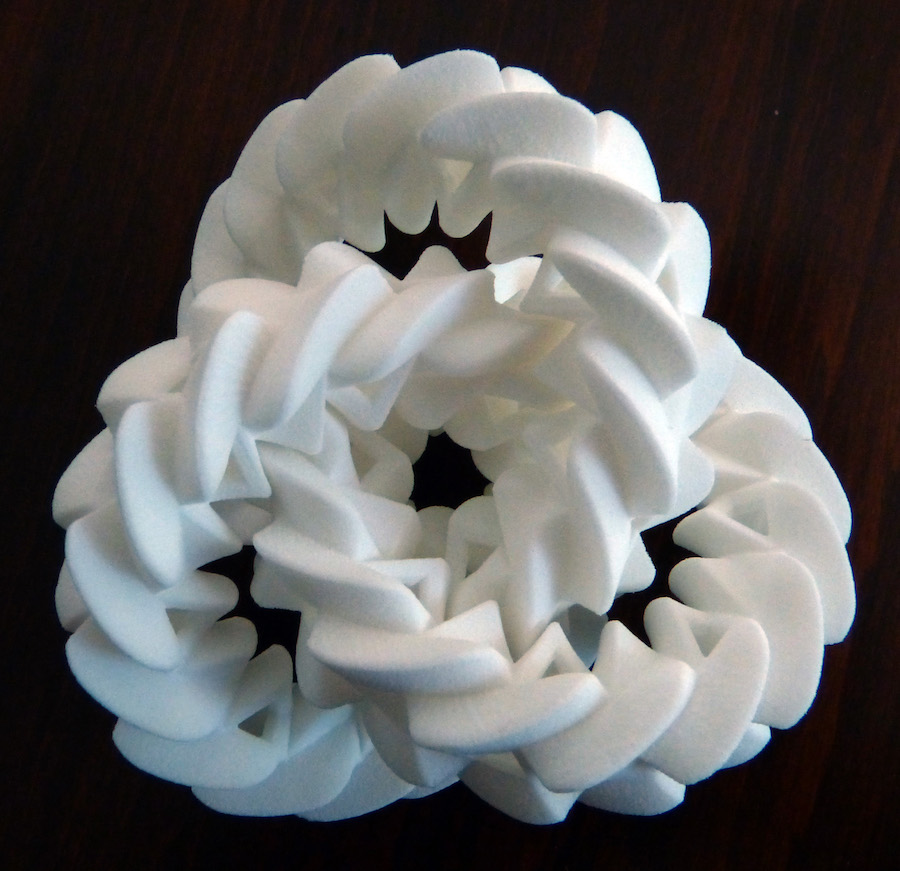
\includegraphics[width=0.65\textwidth]{mechanic trefoil}
        \caption{Mechanisch model van gekoppelde knoopwervel, visueel analoog van traagheid.}
    \end{figure}

    \begin{figure}[h!]
        \centering
        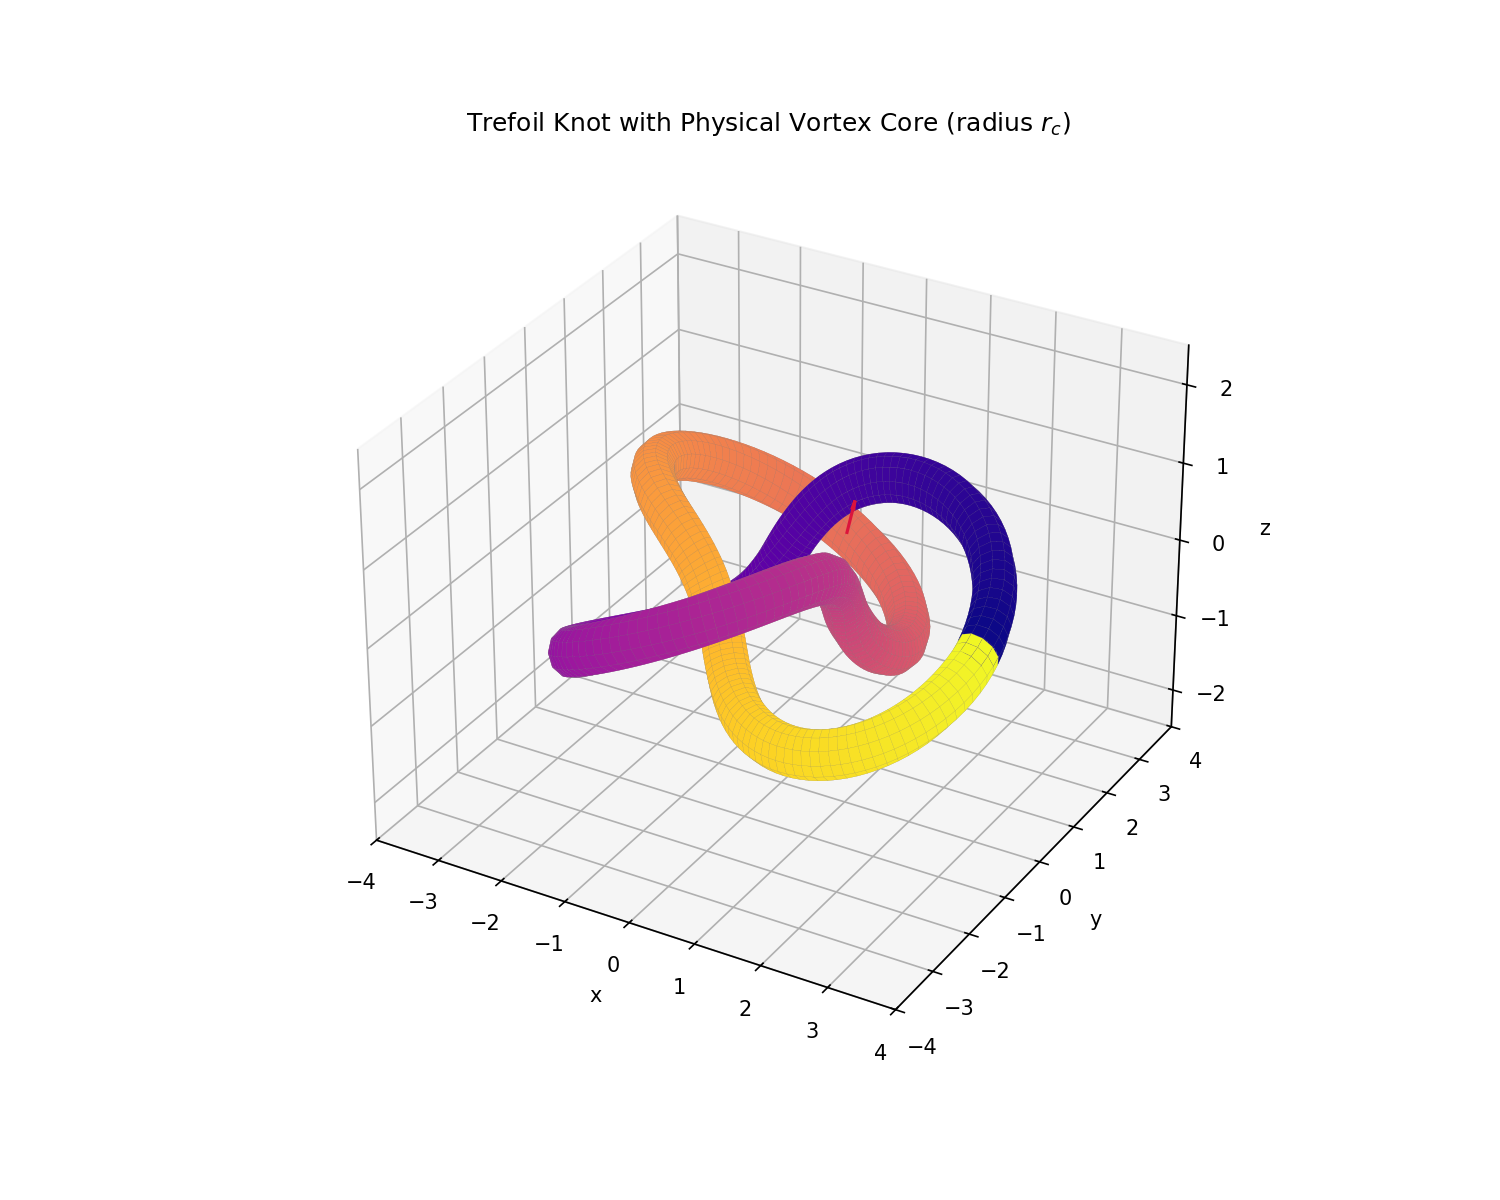
\includegraphics[width=0.8\textwidth]{FatTreFoil.png}
        \caption{Wervelknoop met kernstraal $r_c$, swirl $C_e$ (rode vector).}
    \end{figure}

    \begin{figure}[h!]
        \centering
        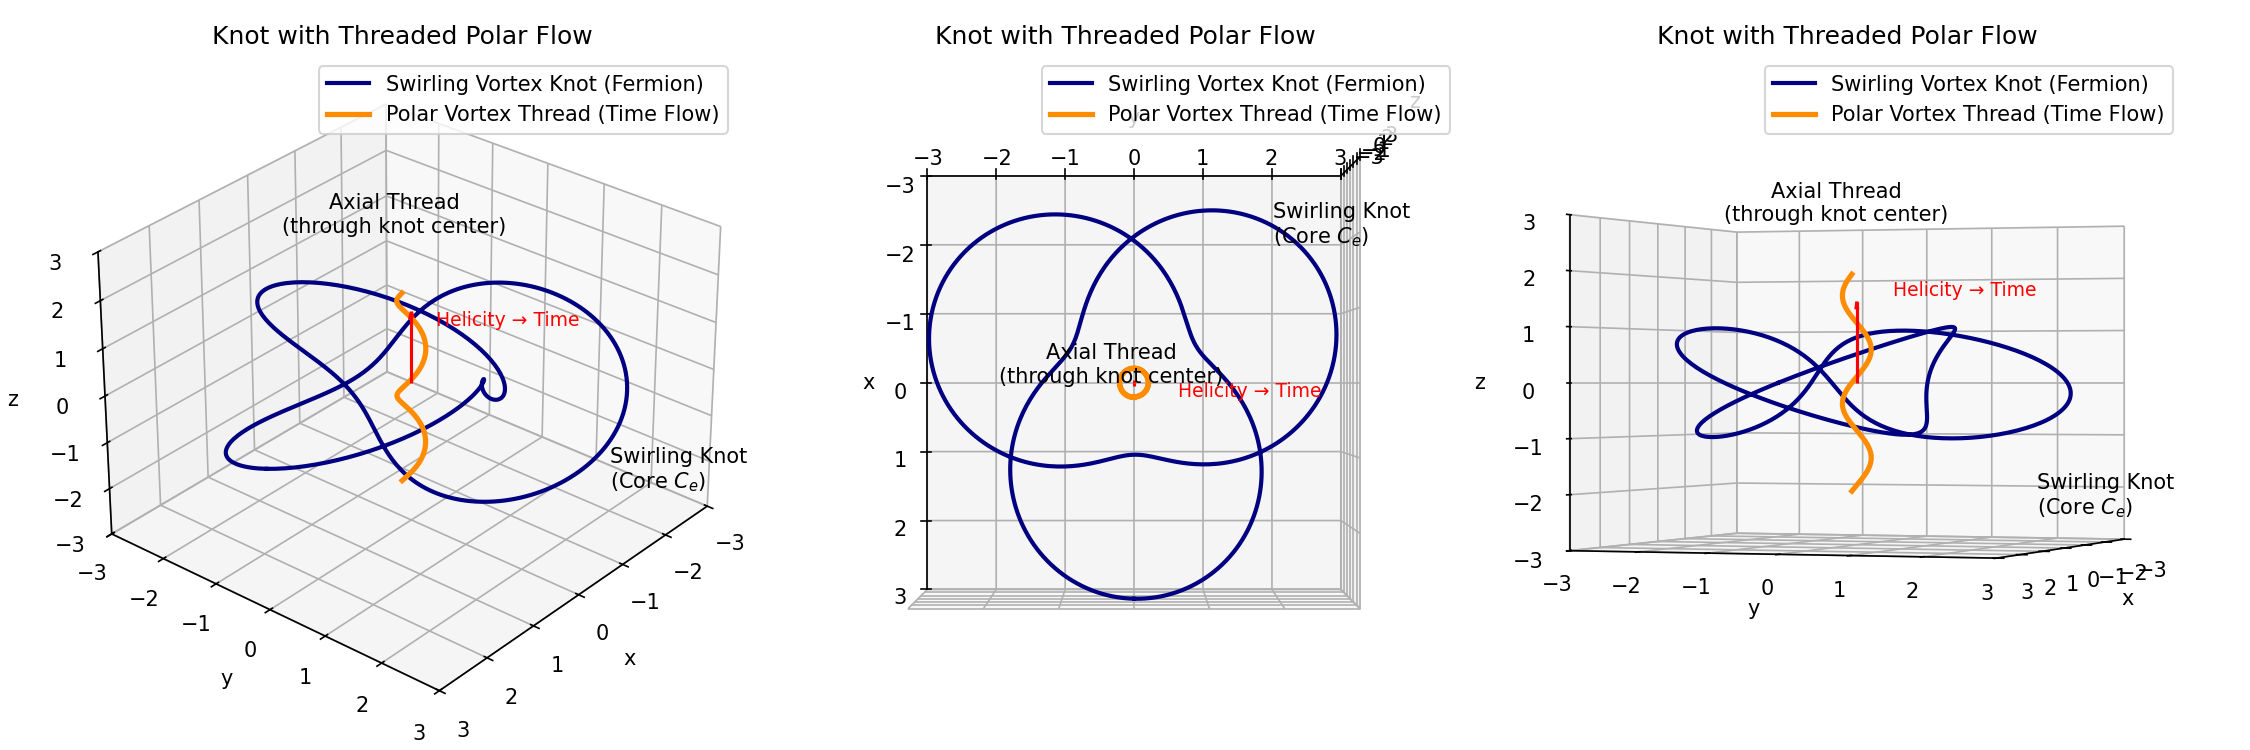
\includegraphics[width=0.98\textwidth]{KnotThreadedPolarFlow.png}
        \caption{Wervelknoop gekoppeld aan polaire draad: tijdsverloop als heliciteitstransport.}
    \end{figure}

    \begin{figure}[h!]
        \centering
        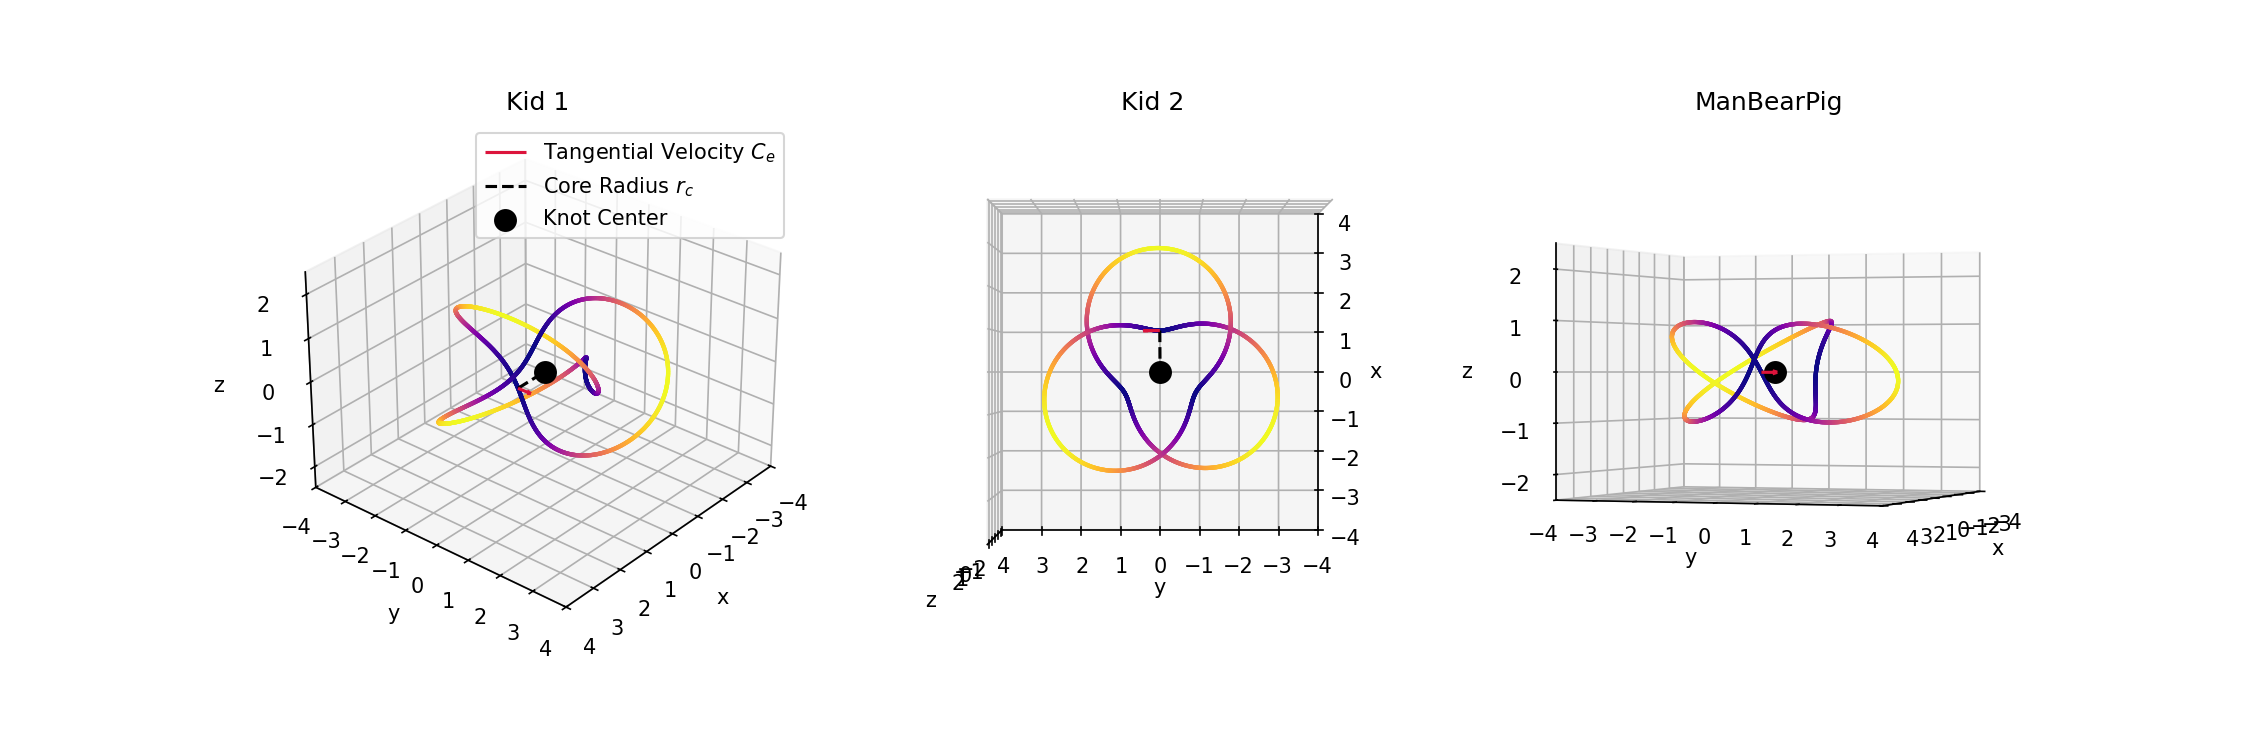
\includegraphics[width=0.95\textwidth]{vortex_knot_diagram.png}
        \caption{Annotatie kernstraal $r_c$ en swirlrichting $C_e$.}
    \end{figure}

    \section{Overzichtstabel: Grootheden in VAM}
    \begin{table}[h!]
        \centering
        \begin{tabular}{|c|l|l|}
            \hline
            \textbf{Symbool} & \textbf{Beschrijving} & \textbf{Eenheid in VAM} \\
            \hline
            $C_e$ & Tangentiële wervelsnelheid & $[L/T]$ \\
            $r_c$ & Kernstraal van wervel & $[L]$ \\
            $\rho_{\ae}$ & Ætherdichtheid & $[M/L^3]$ \\
            $F_{\text{max}}$ & Maximale kracht æther & $[M \cdot L/T^2]$ \\
            $\Gamma$ & Circulatie & $[L^2/T]$ \\
            $\hbar_{\text{VAM}}$ & Wervelmoment & $[M \cdot L^2 / T]$ \\
            $E_0$ & Elementaire energie & $[M \cdot L^2 / T^2]$ \\
            $T_0$ & Elementaire tijd & $[T]$ \\
            $L_0$ & Elementaire lengte & $[L]$ \\
            $M_0$ & Elementaire massa & $[M]$ \\
            \hline
        \end{tabular}
        \caption{Fundamentele grootheden in Vortex Æther Model.}
    \end{table}

    % Canvas inputs

    \section*{Swirl-Coherent Vortex Model of the Galaxy}

In the Vortex \AE ther Model (VAM), mass and gravity are emergent from a network of \emph{chiral vortex knots} (fluid-dynamic analogues of particles) embedded in a superfluid \ae ther. We model the Milky Way as a coherent lattice of such chiral knots -- each knot is a helical vortex (with a definite handedness) that generates a local swirl gravity field and carries an internal clock phase. All knots share a common Swirl Clock phase $S(t)$, meaning their internal rotation states are synchronized across the galactic network\cite{iskandarani2025vam2}.

This synchronization is analogous to phase-locking in coupled oscillators and reflects a single global chirality for the galactic vortex system (a ``swirl domain'' of aligned vortex orientation). Gravitation in this picture arises not from spacetime curvature but from \emph{vorticity-induced pressure gradients} in the \ae ther fluid: the gravitational potential $\Phi_v(\mathbf{r})$ satisfies a Poisson-like equation driven by vorticity magnitude\cite{iskandarani2025vam2}:
\begin{equation}
\nabla^2 \Phi_v(\mathbf{r}) = -\rho_{\ae} |\boldsymbol{\omega}(\mathbf{r})|^2,
\label{eq:swirl-grav}
\end{equation}
where $\boldsymbol{\omega}=\nabla\times \mathbf{v}$ is the local vorticity of the \ae ther flow and $\rho_{\ae}$ its density\cite{iskandarani2025vam2}.

This ``Bernoulli pressure potential'' implies that regions of high swirl (vorticity) produce low pressure (potential wells) that draw in other vortex knots -- effectively reproducing gravity via fluid dynamics. Objects move by aligning with vortex streamlines rather than following geodesics\cite{iskandarani2025vam2}.

Time dilation in this framework emerges from the same swirl dynamics. A local proper time $\tau$ (termed \emph{Chronos-Time}) for an observer inside the vortex field is determined by the swirl kinetic energy. In particular, clock rates slow in regions of high tangential \ae ther velocity $v_{\varphi}$ (i.e., near vortex cores). Quantitatively, one finds an analogous formula to special relativity for the time dilation factor:
\begin{equation}
\frac{d\tau}{dt} = \sqrt{1 - \frac{v_{\varphi}(r)^2}{c^2}},
\label{eq:swirl-time}
\end{equation}
where $v_{\varphi}(r)$ is the local swirl (tangential) speed of the \ae ther at radius $r$ from a vortex core. Near a rotating core, $v_{\varphi}$ is large and $d\tau/dt$ drops below 1 (time runs slow), while far outside the vortex (where $v_{\varphi}\to 0$) the factor approaches unity, recovering normal time flow. This captures gravitational and kinematic time dilation within a unified fluid picture: time slowdown is caused by vortex-induced pressure deficits and swirl energy, rather than spacetime curvature\cite{iskandarani2025vam2}.

Indeed, VAM distinguishes multiple time scales: an absolute universal time $N$ (the \ae ther's global time), the local proper time $\tau$, and an internal Swirl Clock phase $S(t)$ for each vortex\footnote{Iskandarani, O. (2025). \textit{Swirl Clocks and Vorticity-Induced Gravity. Appendix: Temporal Ontology}. doi:10.5281/zenodo.15566336.}. The Swirl Clock tracks the cyclical phase of a knot's rotation and effectively acts as a ``handed'' internal clock tied to vorticity, while $\tau$ measures the cumulative time experienced (akin to an external clock reading).

Crucially, the rate at which a given knot's proper time $\tau$ advances is proportional to the local helicity density (vorticity aligned with velocity) of the \ae ther flow around it:
\begin{equation}
d\tau = \lambda (\mathbf{v}\cdot\boldsymbol{\omega}) dt,
\label{eq:helicity-time}
\end{equation}
for some constant $\lambda$. In other words, helicity $\mathbf{v}\cdot\boldsymbol{\omega}$ -- a measure of swirling twist of flow lines -- effectively drives the passage of proper time for the vortex. A vortex knot ``threads'' time forward by its internal rotation, functioning like a tiny clock whose ticking rate depends on how strongly it stirs the \ae ther.

    \section*{2. Wervelveldenergie en gauge-termen}

Een fundamenteel principe binnen de wervelmechanica is de evolutie van de vorticiteit $\vec{\omega}$ in een ideale vloeistof. Deze wordt beschreven door de derde Helmholtz-wervelstelling:
\[
    \frac{D \vec{\omega}}{Dt} = (\vec{\omega} \cdot \nabla) \vec{v}
\]

waarbij:
- $\vec{\omega} = \nabla \times \vec{v}$ de lokale wervelsterkte is,
- $\vec{v}$ de fluïdumsnelheid,
- $\frac{D}{Dt}$ de materiële afgeleide.

Binnen het Vortex Æther Model wordt aangenomen dat het ætherveld $\vec{v}$ structureel is opgebouwd uit knopen en lussen, en dus dat $\vec{\omega}$ een structureel veld vormt. Dit leidt tot de noodzaak om een veldbeschrijving in te voeren voor $\vec{\omega}$, analoog aan elektromagnetisme.

\subsection*{VAM-analogie met elektromagnetisme}
De klassieke Lagrangiandichtheid van het elektromagnetisch veld is:
\[
    \mathcal{L}_\text{EM} = -\frac{1}{4} F_{\mu\nu} F^{\mu\nu},
\]
waar $F_{\mu\nu} = \partial_\mu A_\nu - \partial_\nu A_\mu$ het veldtensor is.

In VAM introduceren we een \textbf{wervelveld-tensor} $W_{\mu\nu}$ die de antisymmetrische spanningen in het æther encodeert:
\[
    W_{\mu\nu} = \partial_\mu V_\nu - \partial_\nu V_\mu,
\]
waarbij $V_\mu$ het æther-stroompotentiaal is (dimensies van snelheid).

De overeenkomstige energiedichtheid luidt dan:
\[
    \mathcal{L}_\text{wervel} = -\frac{1}{4} W_{\mu\nu} W^{\mu\nu}
\]

Deze term beschrijft:
- Wervelspanning en -energie in het veld zelf
- Propagatie van wervelstructuren
- Koppeling aan knoopconfiguraties in $V_\mu$

\subsection*{Interpretatie en eenheden}
De tensor $W_{\mu\nu}$ heeft eenheidsdimensies van afgeleiden van snelheid:
\[
    [W] = [\partial V] = [1/T] \quad \Rightarrow \quad [\mathcal{L}_\text{wervel}] = [\rho_\text{\ae} C_e^2]
\]

Deze termen zijn direct simuleerbaar in vortexmodellen waarin $\vec{\omega}$ voortkomt uit structurele spanningsvelden die evolueren volgens afgeleide-conservatie.

In het VAM ontstaat veldenergie dus niet uit kwantumfluctuaties, maar uit gestabiliseerde structurele werveling van het æther. De Lagrangiandichtheid volgt hieruit als macroscopisch spanningsveld dat reageert op knoopdichtheid en vorticiteit.
    \section*{3. Wervelmassa als traagheid uit circulatie}

De massa van een knoopwervel in het Vortex Æther Model ontstaat niet als een fundamentele eigenschap, maar als gevolg van circulatie en weerstand tegen vervorming van de æther:

\subsection*{Circulatie als basis voor inertie}
De circulatie van een gesloten wervelpad wordt gegeven door:
\[
    \Gamma = \oint_{\partial S} \vec{v} \cdot d\vec{\ell} = 2\pi r_c C_e
\]
Deze grootheid is behouden in ideale fluïda (Helmholtz-theorema) en vormt een constante parameter voor elke knoopconfiguratie.

De implicatie hiervan is dat bij een gegeven $\Gamma$, elke verandering van $r_c$ (straal van de wervelkern) een overeenkomstige verandering in swirl $C_e$ vereist:
\[
    C_e = \frac{\Gamma}{2\pi r_c}
\]

\subsection*{Afleiding van effectieve massa}
Kinetische energie gekoppeld aan deze swirl is:
\[
    E = \frac{1}{2} \rho_{\ae} C_e^2 V = \frac{1}{2} \rho_{\ae} \left( \frac{\Gamma}{2\pi r_c} \right)^2 \cdot \frac{4}{3}\pi r_c^3
\]
\[
    \Rightarrow E = \frac{\rho_{\ae} \Gamma^2}{6\pi r_c}
\]

Deze energie kunnen we associëren met de klassieke inertieformule $E = \frac{1}{2} m C_e^2$, waaruit een effectieve massa volgt:
\[
    m_\text{eff} = \frac{\rho_{\ae} \Gamma^2}{3\pi r_c C_e^2}
\]

Dit toont dat massa direct voortkomt uit:
- De circulatiekracht $\Gamma$
- De geometrie van de knoop ($r_c$)
- De wervelsnelheid $C_e$

\subsection*{Vergelijking met klassieke inertie}
Ter vergelijking:
\[
    m \sim \frac\text{traagheidsenergie}{C_e^2} \quad \text{vs.} \quad E = m c^2 \text{ in SR}
\]
In VAM is $C_e$ de lokale swirl-constante, en $c$ de propagatiesnelheid van verstoringen. Dat betekent dat massa in VAM **afleidbaar is uit geometrie en behoud** — en niet fundamenteel postulaat.

\subsection*{Fermion-massaterm in Lagrangian}
Met bovenstaande afleiding kunnen we de massaterm van een fermion schrijven als:
\[
    \mathcal{L}_\text{massa} = m_f C_e r_c \cdot \bar{\psi}_f \psi_f
\]
waarbij $m_f$ hier proportioneel is aan $\rho_{\ae}$ en $\Gamma^2$ van de knoopwervel. Dit vervangt de standaard Yukawa-koppeling door een fluïdumeigenschap.
    \section*{4. Druk- en spanningspotentiaal van æthercondensaat}

De vierde bijdrage aan de VAM-Lagrangian betreft de beschrijving van drukspanning en evenwichtstoestanden in het æther. In analoge zin met het Higgsmechanisme wordt dit gemodelleerd via een scalair veld $\phi$ dat de lokale toestand van het æther representeert.

\subsection*{Veldinterpretatie}
Het veld $\phi$ meet de verstoring van het æthervolume als gevolg van een wervelknoop. Bij sterke swirl $C_e$ en hoge vorticiteit $\omega$ zal de lokale druk dalen (Bernoulli-effect), wat zich uit in een verandering van het evenwichtspunt van het æther:
\[
    P_{\text{lokaal}} < P_\infty \Rightarrow \phi \neq 0
\]

\subsection*{Potentiaalvorm en afleiding}
De æthertoestand wordt beschreven door een klassieke potentiaal van de vorm:
\[
    V(\phi) = -\frac{F_{\text{max}}}{r_c} |\phi|^2 + \lambda |\phi|^4
\]

Hierin:
- $\frac{F_{\text{max}}}{r_c}$ is de maximale compressieve spanningsdichtheid van de æther,
- $\lambda$ bepaalt de stijfheid van het systeem tegen overspanning.

De minima van deze potentiaal liggen bij:
\[
    |\phi| = \sqrt{\frac{F_{\text{max}}}{2 \lambda r_c}}
\]
Dit is een stabiele toestand waarin het æther zich herstructureert rond een stabiele knoopconfiguratie.

\subsection*{Vergelijking met Higgsveld}
In standaardveldentheorie is het Higgsveldverhaal:\newline
\centerline{$V(H) = -\mu^2 |H|^2 + \lambda |H|^4$}
waar $\mu^2$ een negatieve massaterm is die spontane symmetriebreking uitlokt.

In VAM komt de breking voort uit reële æthercompressie, waardoor de fysische oorsprong van $\phi$ niet willekeurig is maar voortkomt uit spanningsbalans:
\[
    \frac{dV}{d\phi} = 0 \Rightarrow \text{drukkracht in evenwicht met wervelstructuur}
\]

\subsection*{Lagrangiandichtheid voor het æthercondensaat}
De totale bijdrage aan de Lagrangian voor het spanningsveld luidt:
\[
    \mathcal{L}_{\phi} = -|D_\mu \phi|^2 - V(\phi)
\]
Hierin wordt $D_\mu$ geïnterpreteerd als afgeleide langs de richting van de spanningsverandering in het wervelveld (mogelijk gekoppeld aan $V_\mu$).

Deze term vertegenwoordigt:\newline
• De interne elasticiteit van het æther,\newline
• De manier waarop topologische verstoringen de spanningsverdeling verschuiven,\newline
• En het mechanisme waardoor massatermen voortkomen uit lokale ætherinteractie.

\subsection*{Opmerking over simulatie}
Deze veldvorm en zijn dynamica zijn numeriek simuleerbaar binnen bestaande systemen van klassieke ætherfluïda (bv. op basis van compressiepotentialen), wat experimentele validatie binnen bereik brengt.
    \section*{5. Mapping van SU(3) \texorpdfstring{$\times$}{x} SU(2) \texorpdfstring{$\times$}{x} U(1) naar VAM-wervelgroepen}

De standaardmodel-Lagrangian is gebaseerd op de gaugegroep:
\[
    SU(3)_C \times SU(2)_L \times U(1)_Y
\]
die de kleurinteractie (QCD), de zwakke interactie en elektromagnetisme beschrijven via hun bijbehorende vectorvelden. In het Vortex Æther Model (VAM) bestaan geen abstracte ruimtetijdsymmetrieën — alle krachten en interacties moeten herleid worden tot wervelstructuren en topologische stromingen in een 3D Euclidische æther.

\subsection*{5.1 $U(1)_Y$: Swirlrichting als hyperlading}
De eenvoudigste symmetrie, $U(1)$, correspondeert met het behoud van een fase of draairichting. In VAM krijgt dit een directe fysieke betekenis:
\begin{itemize}
    \item \textbf{Fysische interpretatie:} een rechtlijnige swirl (circulair maar niet geknoopt) in de æther representeert een uniforme draairichting.
    \item \textbf{Lading:} hyperlading $Y$ is dan de chirale swirlrichting (rechts- of linkshandig) binnen een axiaal symmetrisch veld.
    \item \textbf{Vergelijking:} dit modelleert elektromagnetisme als macroscopische swirl zonder topologische knoop.
\end{itemize}

\subsection*{5.2 $SU(2)_L$: Chiraliteit als tweevoudige topologische swirl}
De zwakke wisselwerking is intrinsiek chirale: alleen linkshandige fermionen koppelen aan $SU(2)_L$.
\begin{itemize}
    \item \textbf{VAM-interpretatie:} linkshandige en rechtshandige wervels zijn fysiek niet equivalent — ze vertegenwoordigen swirlvelden die onder lokale compressie verschillen in draairichting bezitten.
    \item \textbf{Twee toestanden:} $SU(2)$ correspondeert met een tweedimensionale swirlrichtingruimte: bijvoorbeeld op- en neerspinnende swirl.
    \item \textbf{Veldkoppeling:} gaugevelden van $SU(2)$ worden geïnterpreteerd als transities tussen deze swirlrichtingen via knoopreconnectie.
\end{itemize}

\subsection*{5.3 $SU(3)_C$: Drievoudige vortexkleur als heliciteitsstructuur}
In het standaardmodel beschrijft $SU(3)_C$ de kleurkracht, werkend via gluonen die kleur verwisselen.
\begin{itemize}
    \item \textbf{VAM-interpretatie:} drie topologisch stabiele swirlconfiguraties (bijvoorbeeld drie orthogonale heliciteitsassen) corresponderen met de drie kleuren (rood, groen, blauw).
    \item \textbf{Gluonen:} wisselwerkingen tussen deze structuren worden geïnterpreteerd als vortexinterferentie en transities in knoopconfiguraties, zoals bij knoop-twist, splitsing of vervorming van de kern.
    \item \textbf{Begrenzing:} kleurconfinement ontstaat omdat losse swirlkleurconfiguraties energetisch instabiel zijn buiten samengestelde knopen.
\end{itemize}

\subsection*{5.4 Wiskundige groepsstructuur binnen VAM}
Hoewel VAM een strikt geometrisch-fluidum model is, blijven de symmetrieën behouden in de zin van bewaarbare toestanden:
\begin{itemize}
    \item Swirlrichting $\rightarrow$ $U(1)$-fasesymmetrie
    \item Axiale transformatie $\rightarrow$ $SU(2)$
    \item Kleurknoopbasis $\rightarrow$ $SU(3)$-structuur in 3D-heliciteit
\end{itemize}

\subsection*{Conclusie}
De gebruikelijke abstracte Lie-groepen van het standaardmodel zijn in VAM fysiek realiseerbaar als swirl-, heliciteit- en knoopstructuren in het æther. Hierdoor kunnen de bekende interacties worden behouden en herleid vanuit fluïdumechanische principes, zonder terug te vallen op extra dimensies of onobserveerbare velden.
    %! Author = omar.iskandarani
%! Date = 5/20/2025
\section{Tijdsklokwerking in Wervelknopen}

In het Vortex \AE ther Model worden stabiele knopen opgevat als de fundamentele bouwstenen van materie. Door hun interne swirl—de tangentiële rotatie \( C_e \) rond een kernstraal \( r_c \)—veroorzaken zij een asymmetrische spanningsverdeling in de omringende \ae ther. Deze asymmetrie resulteert in een **axiale stroming langs de kern**, die functioneel overeenkomt met een voortbewegende tijdsdraad. Hoewel er geen geometrische schroefdraad aanwezig is, gedraagt het systeem zich **alsof de kernstructuur een schroefwerking uitvoert** op de omringende fluïdum.

\paragraph{Kosmische swirloriëntatie.}
Net als magnetische domeinen vertonen wervelknopen een voorkeur voor een globale swirlrichting. In een universum met een dominante draairichting zou het omgekeerd draaien van een knoop (bijvoorbeeld antimaterie?) alleen stabiel zijn in isolatie. Dit zou verklaren waarom antimaterie zeldzaam is, en waarom tijdsoriëntatie consistent is in macroscopische systemen.

\paragraph{Swirl als tijdsdrager.}
De draaiing van de knoopkern induceert een centrale stroom \( \vec{v}_\text{tijd} \) die volgens het VAM-model direct overeenkomt met lokaal tijdsverloop:
\[
    dt_{\text{lokaal}} \propto \frac{dr}{\vec{v} \cdot \vec{\omega}}
\]
De koppeling tussen swirl (\( C_e \)) en de axiale afvoer van heliciteit bepaalt daarmee hoe snel tijd verstrijkt nabij een knoop.

\paragraph{Collectieve tijdsdraadnetwerken.}
Wervelknopen neigen ertoe zich te groeperen langs swirlstromingen—vergelijkbaar met magnetische veldlijnen die ijzervijlsel ordenen. Rond massa’s kunnen zo netwerken van tijdsdraden ontstaan, wat een natuurlijk verklaringsmodel biedt voor:
\begin{itemize}
    \item zwaartekracht als concentratie van swirlstromen;
    \item lokale tijdsdilatatie (zoals bij planeten en sterren);
    \item richting van kosmologische tijdsevolutie.
\end{itemize}

Deze emergente klokwerking is een van de meest fundamentele aspecten van VAM. Het brengt massa, tijd en richting onder in één mechanisme dat volledig afleidbaar is uit werveldynamica, zonder beroep op abstracte ruimte-tijdcurvaturen.

    \bibliographystyle{unsrt}
    \printbibliography

\end{document}